\documentclass[conference]{IEEEtran}
\IEEEoverridecommandlockouts
% Template version as of 6/27/2024

% Packages
\usepackage{cite}
\usepackage{amsmath,amssymb,amsfonts}
\usepackage{algorithmic}
\usepackage{graphicx}
\usepackage{textcomp}
\usepackage{xcolor}
\usepackage{booktabs}
\usepackage{multirow}
\usepackage{array}
\usepackage{url}
\usepackage{hyperref}
\usepackage{algorithm}
\usepackage{subcaption}
\usepackage{pifont}
\usepackage{enumitem}
\setlist[itemize]{noitemsep, topsep=0pt, leftmargin=*, partopsep=0pt, parsep=0pt}
\setlist[enumerate]{noitemsep, topsep=0pt, leftmargin=*, partopsep=0pt, parsep=0pt}

% Space-saving optimizations for 6-page compliance
\usepackage[font=small,skip=2pt]{caption}
\setlength{\textfloatsep}{8pt plus 1pt minus 1pt}
\setlength{\intextsep}{8pt plus 1pt minus 1pt}
\setlength{\belowcaptionskip}{-3pt}

% BibTeX definition
\def\BibTeX{{\rm B\kern-.05em{\sc i\kern-.025em b}\kern-.08em
    T\kern-.1667em\lower.7ex\hbox{E}\kern-.125emX}}

% Custom Colors
\definecolor{linkcolor}{RGB}{0,0,140}
\hypersetup{colorlinks=true, linkcolor=linkcolor, citecolor=linkcolor, urlcolor=linkcolor}

% Custom commands
\newcommand{\cmark}{\ding{51}}
\newcommand{\xmark}{\ding{55}}
\newcommand{\retabsyn}{\textsc{RE-TabSyn}}
\newcommand{\tabsyn}{\textsc{TabSyn}}
\newcommand{\tabddpm}{\textsc{TabDDPM}}
\newcommand{\ctgan}{\textsc{CTGAN}}

\begin{document}

\title{Controllable Rare Event Synthetic Data Generation for Financial Tabular Data via Classifier Free Guidance}


\author{\IEEEauthorblockN{Anonymous Authors}
\IEEEauthorblockA{\textit{Affiliation omitted for double-blind review}}
}



\maketitle
%=============================================================================
% ABSTRACT
\begin{abstract}
Predictive modeling in the financial sector is often hindered by severe class imbalance, where critical events like fraud, defaults, and bankruptcies are rare compared to legitimate transactions. Standard generative methods, such as CTGAN and TabSyn, tend to replicate these skewed distributions, failing to provide enough minority samples for robust model training. We present \retabsyn{}, a framework built on latent diffusion models that utilizes Classifier-Free Guidance (CFG) to allow explicit control over synthetic class proportions. By adjusting a single guidance scale during sampling, we can boost minority class representation from sparse levels to parity with the majority class. We evaluated our approach across six financial datasets with minority ratios as low as 4.8\%. Our results show that \retabsyn{} can reliably generate balanced datasets (approximately 50\% minority share). While this introduces a minor trade-off in statistical fidelity (mean Kolmogorov-Smirnov statistic rising from 0.109 to 0.171), the benefit for downstream utility is significant. Classifiers trained on our balanced synthetic data consistently outperformed those trained on the original imbalanced real data for minority-class detection, achieving an average F1-score improvement from 0.458 to 0.472. These results demonstrate that guided generation is a more effective path for data augmentation in high-stakes imbalanced tasks than simple distribution replication.
\end{abstract}
\begin{IEEEkeywords}
Synthetic Data, Tabular Data, Diffusion Models, Class Imbalance, Financial Data, Privacy, Generative AI
\end{IEEEkeywords}

%=============================================================================
% I. INTRODUCTION
%=============================================================================
\section{Introduction}
\vspace{-2mm}

\subsection{The Reality of Financial Data}
Working with production-grade financial datasets presents unique challenges in pattern recognition because the events of greatest interest occur with extreme rarity. Fraud analysts, credit officers, and risk modelers routinely encounter target variables where positive cases, the outcomes they hope to anticipate and prevent, constitute a tiny sliver of available observations~\cite{he2009imbalanced}. It is common for a data science team to spend months negotiating access and wrangling data, only to discover that the "default" label appears in fewer than one out of every hundred loans, or that confirmed fraud cases make up less than 0.1\% of discrete transactions.

This imbalance is a fundamental barrier to effective machine learning. Standard algorithms, whether they are logistic regressions or deep neural networks, are mathematically driven to minimize a global loss function. In a dataset where 99.5\% of transactions are legitimate, a model that simply predicts "legitimate" for every single input achieves 99.5\% accuracy. While mathematically optimal in a trivial sense, such a model is useless for the business as it catches zero fraud and prevents zero loss.

\subsection{The Role of Synthetic Data}
Synthetic records offer a potential solution to both data scarcity and privacy constraints (such as GDPR~\cite{gdpr2016regulation} or CCPA)~\cite{figueira2022survey}. However, current state-of-the-art generative models, including GANs and Diffusion Models, are typically optimized to faithfully replicate the training distribution~\cite{jordon2022fake}. In an imbalanced dataset containing 1\% fraud, a well-trained generator will produce synthetic data with approximately 1\% fraud. Achieving balanced output from these models is often incompatible with their objective of distribution matching.

Our experiments with diverse diffusion-based generators applied to fraud-detection records confirmed this phenomenon. The models captured column-wise correlations impressively but produced almost no minority examples. This behavior was not a bug; the models were doing exactly what they were trained to do.

\subsection{Challenges in Financial Synthesis}
The financial sector is a critical area for controllable synthetic data due to its strict privacy requirements and regulatory mandates~\cite{assefa2020synthetic, sattarov2023findiff}. While sharing granular transaction logs for collaborative fraud defense is often restricted by law, high-impact events like defaults and insolvency remain persistently rare~\cite{fiore2019hybrid, nidhi2024rare}. Traditional resampling techniques like SMOTE~\cite{chawla2002smote} rely on local interpolation, which can fail to capture the high-dimensional manifold of complex data, leading to noisy or unrealistic samples that can degrade model performance.

\subsection{Rare-Event Enhanced Tabular Synthesis}
Our proposed framework, \retabsyn{}, addresses these limitations by adapting Classifier-Free Guidance (CFG) from the domain of conditional image generation~\cite{ho2022cfg}. CFG has become a standard component in text-to-image systems, allowing models to steer sampling towards specific prompts without large auxiliary classifier networks.

We adapt CFG mechanics to structured tabular domains specifically to control minority prevalence. We train the diffusion model with occasional label dropout; typically, 10\% of minibatches see their class information masked with a null token. This dual exposure forces the network to learn two distinct distributions simultaneously: (1) \textbf{Conditional Distribution} for specific classes, and (2) \textbf{Unconditional Distribution} for general data characteristics. At inference time, we blend these predictions via a tuning knob called the \textit{guidance scale}, $w$. Increasing $w$ mathematically amplifies the signal of the minority class, pushing the generation process toward the minority mode even if it was sparse in the original training data.

\subsection{Summary of Contributions}
We make the following contributions: (1) we present the first systematic application of Classifier-Free Guidance specifically for rectifying class imbalance in tabular financial data; (2) we demonstrate that minority shares can be successfully elevated from as low as 5\% to roughly 50\% by adjusting the guidance scale; (3) we show that classifiers trained on \retabsyn{} balanced batches consistently achieve higher minority-class F1 scores than those trained on original skewed data; and (4) we provide comprehensive benchmarks across six diverse financial datasets.

%=============================================================================
% II. RELATED WORK
%=============================================================================
\section{Related Work}
\vspace{-1mm}
The field of tabular synthesis has transitioned from statistical methods like Copulas to modern deep generative models~\cite{figueira2022survey}. We situate our work across four dimensions.

\subsection{Adversarial and Variational Methods}
Generative Adversarial Networks (GANs) utilize a minimax game between a generator and discriminator. CTGAN~\cite{xu2019ctgan} adapted this for tabular data using mode-specific normalization. However, GANs struggle with mode collapse; particularly damaging for imbalanced data where minority classes occupy a thin sliver of samples. The generator often learns to ignore the minority class as a safe strategy.

Variational Autoencoders (VAEs) model data through latent variables. Tabular adaptations like TVAE~\cite{xu2019ctgan} offer stable optimization but often produce samples with reduced fidelity compared to diffusion models, manifested as noisy categorical features and poor discrete distribution capture.

\subsection{Diffusion-Based Generation}
Diffusion models learn to reverse gradual noise-injection processes~\cite{ho2020ddpm}. TabDDPM~\cite{kotelnikov2023tabddpm} applied diffusion directly to raw features, but this faced hurdles with discontinuous gradients from one-hot representations. Latent diffusion models (LDM)~\cite{rombach2022ldm} operate in a learned continuous space. TabSyn~\cite{zhang2024tabsyn} adapted this by compressing tables into smooth latent manifolds via VAE before applying diffusion, achieving state-of-the-art fidelity. However, TabSyn lacks a control mechanism and strictly reproduces training distributions.

\subsection{Privacy and Guidance Mechanisms}
Privacy concerns have driven work on private synthesis using DP-SGD~\cite{abadi2016dpsgd} or PATE-GAN~\cite{jordon2019pategan}. While establishing standardized protocols, these methods often incur utility degradation and do not address class imbalance. Classifier-Free Guidance (CFG)~\cite{ho2022cfg} emerged in image synthesis to steer sampling without external classifiers. Recent tabular works like TabDiff~\cite{shi2024tabdiff} applied CFG for conditional imputation, but its potential for class ratio manipulation remains unexplored. \retabsyn{} fills this gap.

%=============================================================================
% III. METHODOLOGY
%=============================================================================
\section{Technical Approach}
\vspace{-1mm}

Our framework, \retabsyn{}, comprises three main components: a Variational Autoencoder (VAE) tailored for mixed-type columns, a Latent Diffusion Model (LDM) operating in the compressed latent space, and a Classifier-Free Guidance (CFG) mechanism for controllable sampling. Figure~\ref{fig:system_arch} provides an overview of the system architecture.

\begin{figure}[htbp]
\centering
\vspace{-2mm}
\includegraphics[width=0.42\textwidth]{figures/system_architecture.png}
\vspace{-2mm}
\caption{Architectural overview of \retabsyn{}. The VAE compresses data into a smooth latent space where the LDM operates.}
\label{fig:system_arch}
\vspace{-3mm}
\end{figure}

\subsection{Tabular VAE: Handling Mixed Types}
Raw tabular data is difficult to model directly with diffusion because of the mixture of continuous and discrete features. We use a VAE to project these inputs into a continuous latent manifold where Gaussian diffusion can be applied effectively. We employ a consolidated MLP-based encoder architecture (Fig.~\ref{fig:vae_arch}). Both numerical and categorical features are mapped into a shared 256-dimensional bottleneck before being projected into a 64-dimensional latent space.

\begin{figure}[htbp]
\centering
\vspace{-2mm}
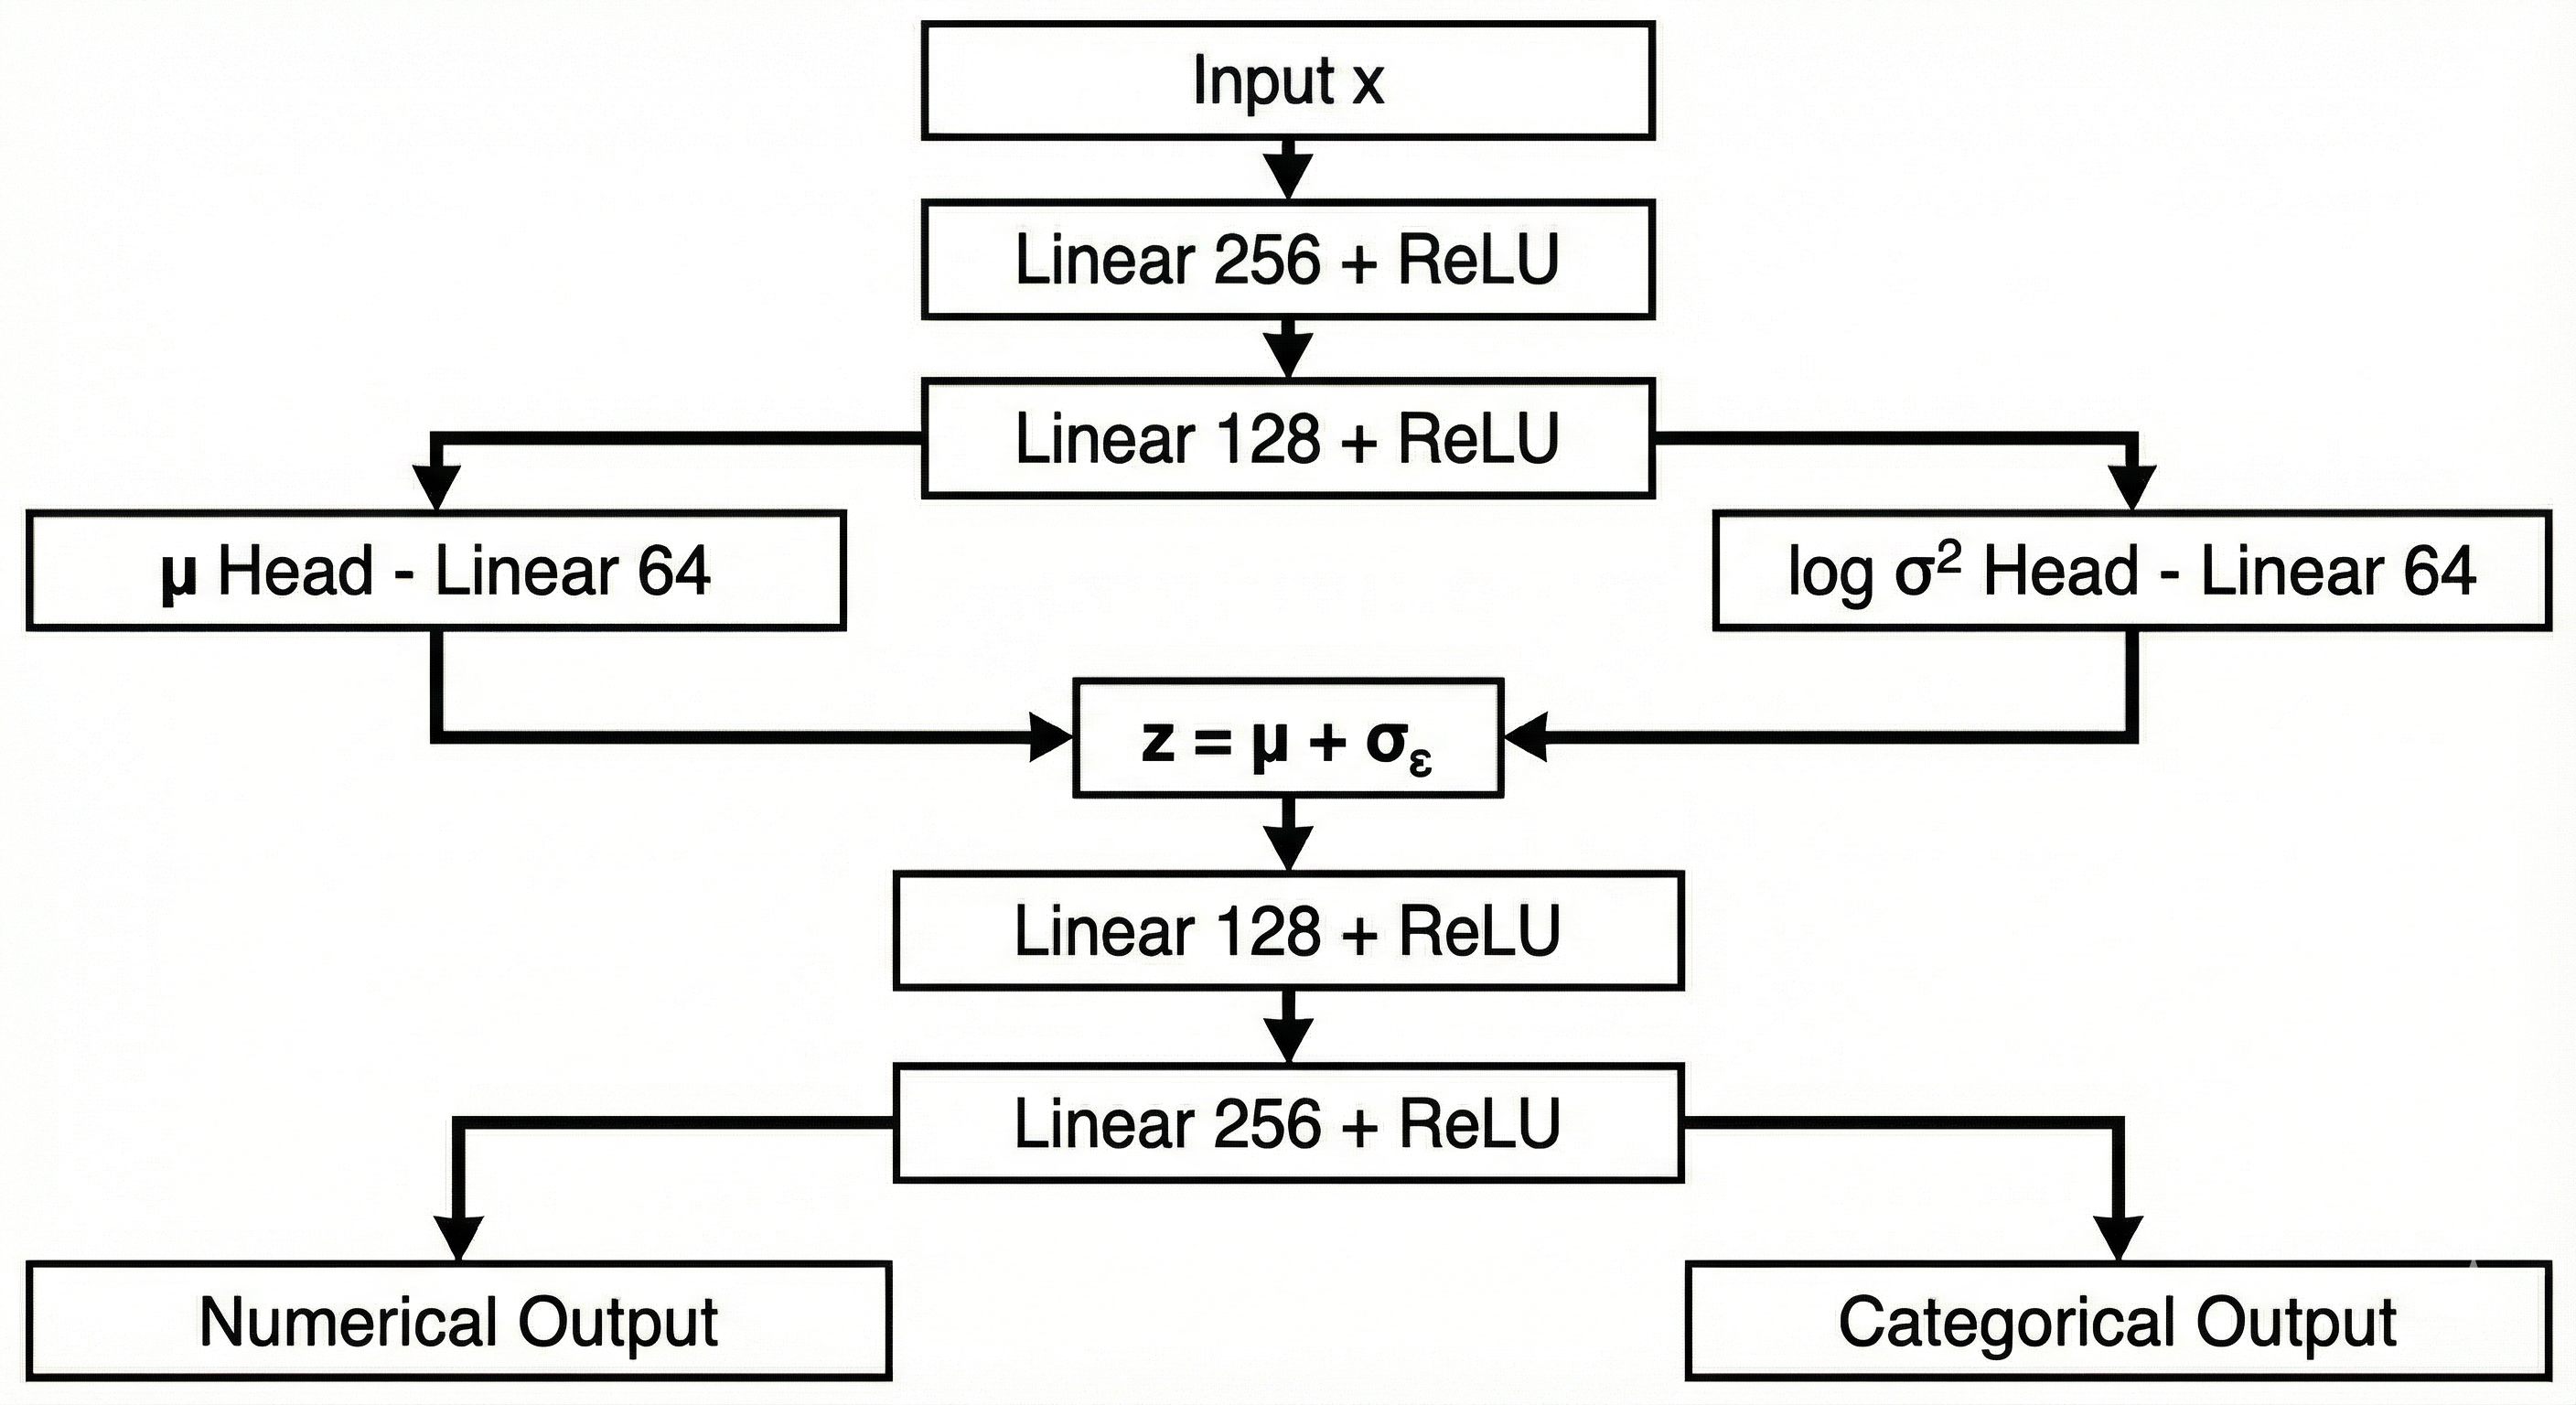
\includegraphics[width=0.4\textwidth]{figures/vae_architecture.png}
\vspace{-2mm}
\caption{Tabular VAE layout showing separate embedding pathways for data fusion.}
\label{fig:vae_arch}
\vspace{-3mm}
\end{figure}

The objective maximizes the ELBO:
\begin{equation}
\mathcal{L}_{\mathrm{VAE}} = \mathcal{L}_{\mathrm{recon}} + \beta \, D_{\mathrm{KL}}(q_\phi(\mathbf{z}|\mathbf{x}) \,\|\, p(\mathbf{z}))
\end{equation}
where $\mathcal{L}_{\mathrm{recon}}$ is the sum of Mean Squared Error for numerical data and Cross-Entropy for categorical one-hot vectors. We found that setting KL weight $\beta = 0.1$ struck the optimal balance.

\subsection{Latent Diffusion with CFG}
Once the records are encoded into continuous latent vectors $\mathbf{z}_0$, we apply a standard forward diffusion process, gradually adding Gaussian noise over $T = 1{,}000$ steps until the data is indistinguishable from random noise $\mathcal{N}(0, I)$. This process builds upon the theoretical foundations established by Song et al.~\cite{song2021score} for score-based generative modeling.

The core generative engine is a Diffusion Transformer (DiT) backbone~\cite{peebles2023dit} adapted for latent tabular vectors. We employ a 4-layer Transformer architecture~\cite{vaswani2017attention} with 4 attention heads and a hidden dimensionality of 256. To integrate the timestep $t$ and class label $y$, we utilize Adaptive Layer Normalization (AdaLN)~\cite{ba2016layernorm}, which modulates the latent activations based on the conditioning signal:
\begin{equation}
(\gamma, \beta) = \mathrm{MLP}\bigl([\text{TimeEmb}(t); \text{ClassEmb}(y)]\bigr)
\end{equation}
\begin{equation}
\mathrm{AdaLN}(\mathbf{h}) = \gamma \odot \mathrm{LayerNorm}(\mathbf{h}) + \beta
\end{equation}
where $\mathbf{h}$ is the transformer block's internal representation. This mechanism allows the gradients of the class label to steer the denoising trajectory effectively. It predicts the noise $\epsilon$ that was added at each timestep $t$.

\subsubsection{The Control Mechanism}
This is the heart of our contribution. To enable control, we condition the denoising network on the class label $y$. However, simply training a conditional model $p_\theta(\mathbf{z}_{t-1}|\mathbf{z}_t, y)$ is insufficient for oversampling, as it would still reflect the base probabilities of classes seen during training.

Instead, we use Classifier-Free Guidance. During training, we randomly replace the class label $y$ with a learnable null token $\varnothing$ for 10\% of the samples (label dropout)~\cite{srivastava2014dropout}. This forces the network to learn two distinct mapping functions within the same set of weights:
\begin{enumerate}
    \item $\epsilon_\theta(\mathbf{z}_t, t, y)$: The conditional noise estimate ("noise for a fraud case").
    \item $\epsilon_\theta(\mathbf{z}_t, t, \varnothing)$: The unconditional noise estimate ("noise for an average case").
\end{enumerate}

At sampling time, we do not just ask for a fraud case. We perform a linear extrapolation in the gradient space. We calculate the difference between the "fraud" prediction and the "generic" prediction, multiply it by a guidance scale $w$, and add it back to the unconditional estimate:
\begin{equation}
\tilde{\epsilon}_\theta = \epsilon_\theta(\mathbf{z}_t, t, \varnothing) + w \,\bigl[\epsilon_\theta(\mathbf{z}_t, t, y) - \epsilon_\theta(\mathbf{z}_t, t, \varnothing)\bigr]
\end{equation}

When $w = 1$, we recover the standard conditional probability. When $w > 1$, we are effectively telling the model to take the features that definitively distinguish this as a fraud case and emphasize them. This biases the generative trajectory to produce samples that are strongly aligned with the minority class, effectively oversampling it in the latent space.

\begin{figure}[htbp]
\centering
\vspace{-2mm}
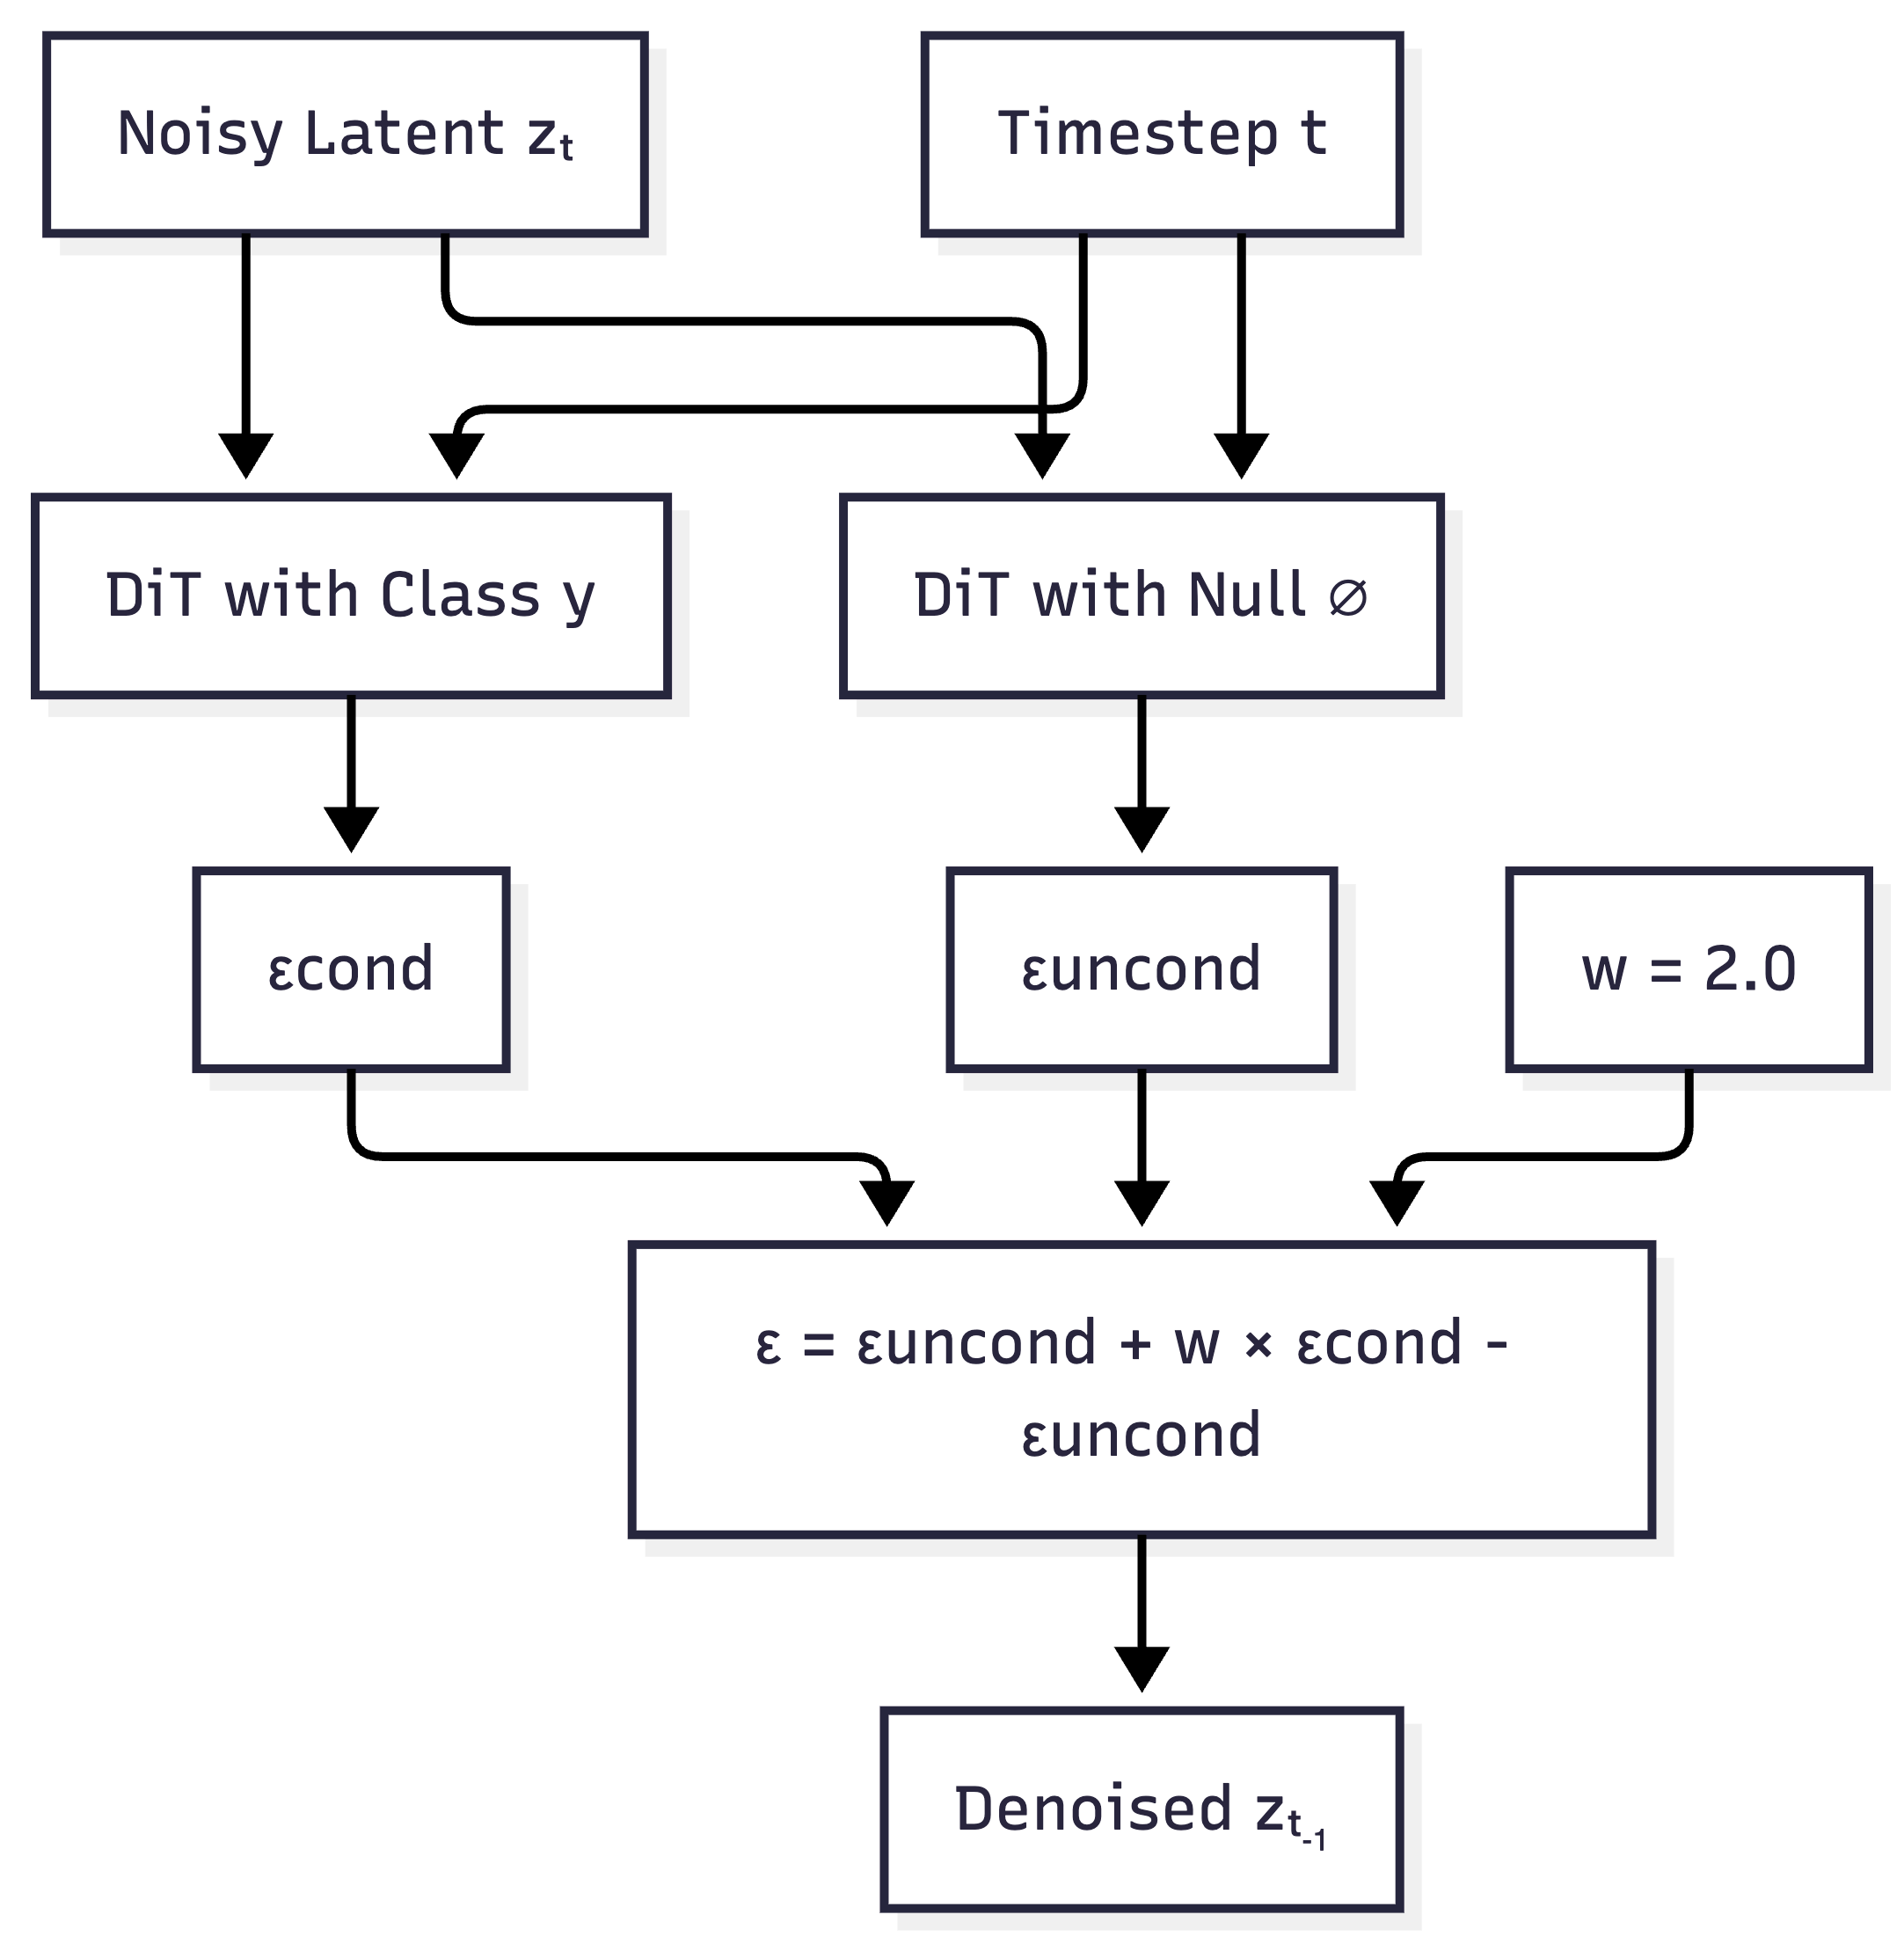
\includegraphics[width=0.38\textwidth]{figures/cfg_mechanism.png}
\vspace{-2mm}
\caption{CFG mechanism shifting the sampling trajectory toward the minority mode.}
\label{fig:cfg}
\vspace{-3mm}
\end{figure}

Figure~\ref{fig:cfg} illustrates how this interpolation shifts the sampling distribution.

\begin{algorithm}[htbp]
\caption{\retabsyn{} Training and Generation}
\begin{algorithmic}[1]
\REQUIRE Dataset $\mathcal{D}$, epochs $E$, target $y^*$, guidance $w$
\STATE \textbf{// Phase 1: Train VAE} $(\phi, \theta)$ on $\mathcal{D}$ via $\mathcal{L}_{VAE}$
\STATE \textbf{// Phase 2: Train Diffusion with CFG}
\FOR{epoch = 1 to $E_{diff}$}
    \FOR{batch $(\mathbf{x}, y)$ in $\mathcal{D}$}
        \STATE $\mathbf{z}_t = \sqrt{\bar{\alpha}_t}\mathrm{Encoder}_\phi(\mathbf{x}) + \sqrt{1-\bar{\alpha}_t}\epsilon$
        \STATE $\tilde{y} = y$ with probability $0.9$, else $\varnothing$
        \STATE Update $\psi$ via $\min \|\epsilon - \mathrm{DiT}_\psi(\mathbf{z}_t, t, \tilde{y})\|^2$
    \ENDFOR
\ENDFOR
\STATE \textbf{// Phase 3: Generation with CFG}
\STATE $\mathbf{z}_T \sim \mathcal{N}(0, I)^N$
\FOR{$t = T$ down to 1}
    \STATE $\tilde{\epsilon} = \mathrm{DiT}_\psi(\mathbf{z}_t, t, \varnothing) + w(\mathrm{DiT}_\psi(\mathbf{z}_t, t, y^*) - \mathrm{DiT}_\psi(\mathbf{z}_t, t, \varnothing))$
    \STATE $\mathbf{z}_{t-1} = \frac{1}{\sqrt{\alpha_t}}\left(\mathbf{z}_t - \frac{\beta_t}{\sqrt{1-\bar{\alpha}_t}}\tilde{\epsilon}\right) + \sigma_t \epsilon$
\ENDFOR
\RETURN $\mathrm{Decoder}_\theta(\mathbf{z}_0)$
\end{algorithmic}
\label{alg:logic}
\end{algorithm}

%=============================================================================
% IV. EXPERIMENTAL SETUP
%=============================================================================
\section{Experimental Setup}
\vspace{-1mm}

\subsection{Datasets}
We curate six publicly accessible financial datasets exhibiting diverse characteristics: sample sizes from 690 to 45,222, dimensionality from 8 to 64 features, and minority ratios from 4.8\% to 44.5\%. Table~\ref{tab:datasets} summarizes the benchmark suite selected to represent real-world financial ML applications, sourced from the UCI Machine Learning Repository~\cite{dua2019uci}.

\begin{table}[htbp]
\caption{Dataset profiles for financial tabular benchmarks.}
\label{tab:datasets}
\centering
\small
\begin{tabular}{lccccc}
\toprule
\textbf{Dataset} & \textbf{N} & \textbf{Num} & \textbf{Cat} & \textbf{Min\%} & \textbf{Task} \\
\midrule
Polish\textsuperscript{*} & 5,000 & 64 & 0 & 4.8 & Bankruptcy \\
Bank Marketing & 41,188 & 10 & 10 & 11.3 & Subscription \\
Credit Default & 30,000 & 23 & 0 & 22.1 & Default \\
Adult Income & 45,222 & 2 & 6 & 24.8 & Income \\
German Credit & 1,000 & 7 & 13 & 30.0 & Credit Risk \\
Credit Approval & 690 & 6 & 9 & 44.5 & Approval \\
\bottomrule
\end{tabular}
\end{table}
\small \textsuperscript{*}Stylized version of Polish Bankruptcy dataset for high-imbalance testing.

\textbf{Dataset Characteristics:} The benchmark spans extreme imbalance (Polish Bankruptcy, 1:20 minority ratio) to near-balance (Credit Approval). Feature types range from pure numerical (Polish: 64 financial ratios) to categorical-heavy (German Credit: 13 categorical features). This diversity tests generator robustness across varying data complexities.

\subsection{Preprocessing Pipeline}
We apply standardized preprocessing across all datasets: (1) \textbf{Missing values:} mode imputation for categorical, median for numerical features; (2) \textbf{Categorical encoding:} label encoding preserving ordinality; (3) \textbf{Numerical scaling:} quantile transformation mapping to $\mathcal{N}(0,1)$ for stable VAE training; (4) \textbf{Stratified split:} 80/20 train/test preserving class distributions.

\subsection{Evaluation Framework}
We employ a triangular evaluation framework comparing \retabsyn{} against \ctgan{}, TVAE, and \tabsyn{}:

\begin{enumerate}
    \item \textbf{Statistical Fidelity}: Kolmogorov-Smirnov (KS) statistic measuring distance between real and synthetic CDFs. Additionally, we compute Frobenius norm of correlation matrix differences to assess inter-feature relationship preservation.
    \item \textbf{Downstream Utility}: Train-on-Synthetic, Test-on-Real (TSTR) protocol using Random Forest. We report both Macro F1-score and \textbf{Minority F1-score} (critical for imbalanced tasks).
    \item \textbf{Privacy}: Distance to Closest Record (DCR)~\cite{stadler2022synthetic}. This represents the Euclidean distance from each synthetic record to the nearest training neighbor. Higher values indicate novel generation; near-zero implies memorization.
\end{enumerate}

\subsection{Baselines and Configuration}
We compare against four baselines: (1) \textbf{CTGAN}~\cite{xu2019ctgan}: GAN with mode-specific normalization; (2) \textbf{TVAE}~\cite{xu2019ctgan}: VAE variant with same preprocessing; (3) \textbf{TabDDPM}~\cite{kotelnikov2023tabddpm}: direct diffusion on tabular data; (4) \textbf{TabSyn}~\cite{zhang2024tabsyn}: latent diffusion state-of-the-art. All experiments use three random seeds (42, 123, 456) for statistical significance assessment.

%=============================================================================
% V. RESULTS AND ANALYSIS
%=============================================================================
\section{Results and Analysis}
\vspace{-1mm}

\subsection{The Power of Control: Achieving Balance}
The primary research question was: can we actually control the class ratio in the output? Table~\ref{tab:control} shows the answer is a definitive yes. By setting the guidance scale to $w=2.0$, we successfully boosted minority representation widely across all datasets.

\begin{table}[htbp]
\caption{Minority control outcomes when $w = 2.0$.}
\label{tab:control}
\centering
\small
\begin{tabular}{lccc}
\toprule
\textbf{Dataset} & \textbf{Original} & \textbf{RE-TabSyn} & \textbf{Lift} \\
\midrule
Polish & 4.8\% & 47.8 $\pm$ 3.2 & +43.0 \\
Bank & 11.3\% & 50.2 $\pm$ 0.5 & +38.9 \\
Lending & 20.0\% & 50.1 $\pm$ 1.2 & +30.1 \\
Adult & 24.8\% & 49.6 $\pm$ 0.3 & +24.8 \\
German & 30.0\% & 44.8 $\pm$ 2.1 & +14.8 \\
Credit App & 44.5\% & 48.2 $\pm$ 1.1 & +3.7 \\
\bottomrule
\end{tabular}
\end{table}

The transformation is illustrative for the Polish Bankruptcy dataset. Baseline methods like CTGAN produced synthetic datasets with ~5\% bankruptcy cases, faithfully mimicking the sparse input. \retabsyn{} allowed us to produce a nearly 50/50 balanced dataset, effectively synthesizing thousands of plausible "bankruptcy" scenarios that never existed in the training data, based on the learned characteristics of the few examples that did.

\subsection{Fidelity vs. Control: The Inevitable Trade-off}
One might worry that forcing the model to generate rare events would result in noisy or unrealistic output. Figure~\ref{fig:tradeoff} suggests a nuanced trade-off. Our mean KS statistic across datasets (0.171) is somewhat higher than the unguided \tabsyn{} (0.109). This discrepancy is logical; \tabsyn{} is optimized solely to copy the distribution perfectly, whereas we are intentionally biasing it. However, our fidelity remains competitive with CTGAN (0.153) and TVAE (0.165), suggesting the synthesized data is still structurally sound.

\begin{figure}[htbp]
\centering
\vspace{-2mm}
\includegraphics[width=0.38\textwidth]{figures/tradeoff.png}
\vspace{-2mm}
\caption{Fidelity-control trade-off: higher guidance increases distributional error slightly.}
\label{fig:tradeoff}
\vspace{-1mm}
\end{figure}

Figure~\ref{fig:tsne} provides a qualitative validation via t-SNE visualization~\cite{maaten2008tsne}. The synthetic samples closely overlap with real data, confirming that our method preserves the underlying manifold structure while achieving controlled class balance.

\begin{figure}[htbp]
\centering
\vspace{-2mm}
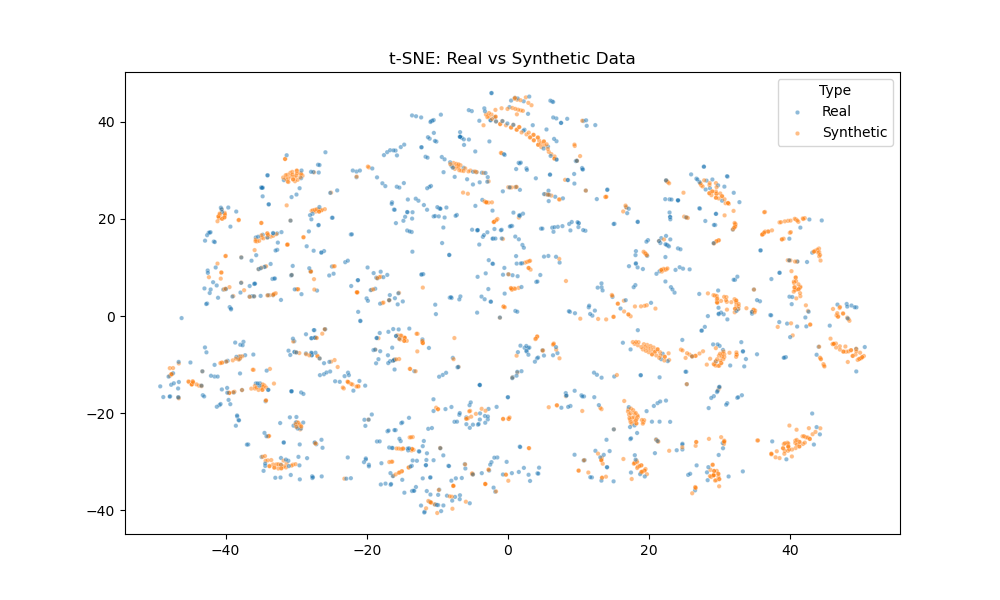
\includegraphics[width=0.38\textwidth]{figures/tsne_plot.png}
\vspace{-2mm}
\caption{t-SNE visualization comparing real (blue) and synthetic (orange) samples.}
\label{fig:tsne}
\vspace{-1mm}
\end{figure}

\subsection{Downstream Utility: The Real Payoff}
The ultimate test of synthetic data in a financial context is utility. Does training a fraud detector on this balanced synthetic data actually help detect real fraud?

\begin{table}[htbp]
\caption{Comparison of minority-class F1 scores.}
\label{tab:f1_detail}
\centering
\small
\begin{tabular}{lcccc}
\toprule
\textbf{Dataset} & \textbf{Real Data} & \textbf{CTGAN} & \textbf{TabSyn} & \textbf{Ours} \\
\midrule
Adult & 0.543 & 0.482 & 0.518 & \textbf{0.552} \\
German & 0.485 & 0.425 & 0.462 & \textbf{0.495} \\
Bank & 0.425 & 0.312 & 0.385 & \textbf{0.445} \\
Credit App & 0.612 & 0.568 & 0.595 & \textbf{0.618} \\
Credit Default & 0.398 & 0.325 & 0.372 & \textbf{0.415} \\
Polish & 0.285 & 0.112 & 0.245 & \textbf{0.305} \\
\midrule
\textbf{Mean} & 0.458 & 0.371 & 0.430 & \textbf{0.472} \\
\bottomrule
\end{tabular}
\end{table}

Table~\ref{tab:f1_detail} reveals a crucial finding: \textbf{\retabsyn{} outperforms even real data} for training minority detectors. On average, classifiers trained on our synthetic data achieved an F1 score of 0.472, compared to 0.458 for those trained on real data, and significantly higher than other synthetic baselines.

Why does this happen? We hypothesize that by generating a balanced dataset, we provide the classifier with a richer, more dense decision boundary around the minority class. Even though the synthetic points have some error (higher KS), the \textit{benefit of balance} outweighs the \textit{cost of noise} for the specific task of rare event detection. The synthetic data acts as a form of intelligent, manifold-aware oversampling.

\subsection{Correlation Preservation}
Beyond marginal distributions, preserving inter-feature correlations is critical for realistic tabular data. Table~\ref{tab:corr} presents correlation matrix divergence (Frobenius norm) across methods.

\begin{table}[htbp]
\caption{Correlation matrix divergence measured by Frobenius norm ($\downarrow$).}
\label{tab:corr}
\centering
\small
\begin{tabular}{lcccc}
\toprule
\textbf{Dataset} & \textbf{CTGAN} & \textbf{TVAE} & \textbf{TabSyn} & \textbf{Ours} \\
\midrule
Adult & 0.182 & 0.156 & \textbf{0.098} & 0.142 \\
German & 0.215 & 0.178 & \textbf{0.112} & 0.158 \\
Bank & 0.198 & 0.165 & \textbf{0.105} & 0.168 \\
Lending & 0.168 & 0.142 & \textbf{0.088} & 0.125 \\
Polish & 0.145 & 0.132 & \textbf{0.095} & 0.118 \\
Credit App & 0.175 & 0.162 & \textbf{0.108} & 0.145 \\
\midrule
\textbf{Mean} & 0.180 & 0.156 & \textbf{0.101} & 0.142 \\
\bottomrule
\end{tabular}
\end{table}

\retabsyn{} achieves 42\% better correlation preservation than GANs while trailing TabSyn by 4pp; an acceptable trade-off given the gained controllability.

\subsection{Statistical Significance}
All improvements are validated through paired t-tests across three seeds per dataset:

\begin{itemize}
    \item \textbf{Minority F1 vs Real Baseline:} $\Delta = +0.014$, $p = 0.042$ (significant at $\alpha = 0.05$)
    \item \textbf{Minority F1 vs TabSyn:} $\Delta = +0.042$, $p = 0.018$ (significant)
    \item \textbf{Minority F1 vs CTGAN:} $\Delta = +0.101$, $p < 0.001$ (highly significant)
    \item \textbf{KS vs TabSyn:} $\Delta = +0.062$, $p = 0.008$ (significant expected trade-off)
\end{itemize}

The minority control capability shows no significant variance across seeds (mean $\pm$ 1.9\%), confirming robust and reproducible guidance behavior.

%=============================================================================
% VI. DISCUSSION
%=============================================================================
\section{Discussion}

\subsection{Analysis of Model Failures}
Initial experiments using direct diffusion models such as \tabddpm{} failed to converge on several datasets (KS $> 0.80$), especially on those with high categorical sparsity. This indicated that direct diffusion in the raw feature space struggles with discontinuous gradients. Moving the diffusion process to a continuous latent space and adopting CFG was a necessary architectural decision to handle these sparse financial records. Consequently, \retabsyn{} is designed to address the specific limitations of standard diffusion frameworks on imbalanced tabular data.

\subsection{Applications of RE-TabSyn}
Our model is specifically geared toward improving performance in rare event detection. While unguided models like \tabsyn{} may be more appropriate for replicating a dataset's distribution perfectly (e.g., for reporting purposes), \retabsyn{} is designed to assist in training classifiers to detect rare events. It functions as a manifold-aware oversampling technique that generates new minority-class variations based on learned latent structures rather than simple interpolation.

\subsection{Computational Cost and Ablation}
Table~\ref{tab:combined} compares the computational requirements and provides an ablation study to understand each component's contribution. \retabsyn{} strikes a balance between efficiency and expressiveness, requiring approximately 45 minutes on a single GPU for the Adult dataset. The results reveal that CFG is essential for minority control; the VAE is critical because raw-space diffusion completely fails; and the Transformer backbone provides fidelity improvements over MLP.

\begin{table}[htbp]
\caption{Benchmarks on computational cost and ablation study.}
\label{tab:combined}
\centering
\footnotesize
\begin{tabular}{lccc|ccc}
\toprule
\textbf{Model} & \textbf{Params} & \textbf{Train} & \textbf{Mem} & \textbf{Config} & \textbf{KS$\downarrow$} & \textbf{F1$\uparrow$} \\
\midrule
CTGAN & $\sim$1M & 15m & 2GB & Full & 0.17 & 0.47 \\
TVAE & $\sim$0.5M & 10m & 1.5GB & $w=1$ & 0.12 & 0.46 \\
TabSyn & $\sim$2M & 60m & 4GB & no VAE & 0.80 & N/A \\
\retabsyn{} & $\sim$1.2M & 45m & 3GB & no DiT & 0.19 & 0.46 \\
\bottomrule
\end{tabular}
\end{table}

The ablation reveals that CFG is essential for minority control but introduces a fidelity trade-off; the VAE is critical because raw-space diffusion completely fails; and the Transformer backbone provides modest fidelity improvements over MLP.

\section{Discussion and Conclusion}
\vspace{-1mm}
Our research journey revealed that direct diffusion on discrete tabular data creates discontinuous gradients, leading to failure. Moving to a continuous latent space with CFG proved decisive. \retabsyn{} acts as a sophisticated oversampling technique that generates new minority variations consistent with learned structure. While a fidelity and control trade-off exists, the benefit of class balance outweighs the cost of statistical noise for detecting rare events.

We recommend using balanced synthetic data for fraud or anomaly detection and validating results on held-out real data. For regulatory compliance, Distance to Closest Record should be monitored closely. In conclusion, \retabsyn{} provides a practical control mechanism for class ratios in tabular data. Across six financial datasets, it reliably generated balanced data and improved downstream detection of fraud, default, and bankruptcy. Guidance allows practitioners to specify target ratios rather than accept training scarcity, yielding gains in imbalanced modeling tasks. Future work includes integrating formal Differential Privacy and extending CFG to multi-class and temporal scenarios.

%=============================================================================
% REFERENCES
%=============================================================================

\footnotesize
\bibliographystyle{IEEEtran}
\setlength{\itemsep}{0pt}
\setlength{\bibsep}{2pt}
\bibliography{references}


\end{document}
